%Hauptdokumentation der L�sung
\NeedsTeXFormat{LaTeX2e}

\documentclass[a4paper,oneside,abstract]{scrreprt}

\usepackage[left=2cm,right=2cm,top=1cm,bottom=2cm,includeheadfoot]{geometry}

\usepackage{ae}
\usepackage{ngerman}				% neue deutsche Rechtschreibung
\usepackage[ngerman]{babel}			% "Table of Contents" --> "Inhaltsverzeichnis"

\usepackage[T1]{fontenc}			% Fontkodierung auf T1-Format
\usepackage{graphicx}				% Bilder
\usepackage{fancyhdr}				% Kopf- und Fusszeilen
\usepackage{lastpage}				% Anzahl gesamte Seiten
\usepackage{hyperref}				% f\"ur Hyperlinks
\usepackage{array}					% f\"ur Tabellen (tabular Umgebung)
\usepackage{listings}				% Quellcodeausgabe
\usepackage{supertabular}			% f\"ur Tabellen \"uber mehrere Seiten
\usepackage{verbatim}	
\usepackage[applemac]{inputenc}
\usepackage{cite}
\usepackage{color}					% f�r Farben

% definition f�r Farben
\definecolor{LinkColor}{rgb}{0,0,0.5}
\hypersetup{
	colorlinks=true,				% definition der Links im PDF
	linkcolor=LinkColor,
	citecolor=LinkColor,
	filecolor=LinkColor,
	menucolor=LinkColor,
	pagecolor=LinkColor,
	urlcolor=LinkColor
}


\newcommand{\titel}{Spektrometer App}
\newcommand{\doctype}{Bachelor Thesis}
\newcommand{\untertitel}{Anbindung Spektrometer an mobiles Device}
\newcommand{\datum}{\today}
\newcommand{\autorA}{Andreas L�scher}
\newcommand{\autorB}{Raphael Bolliger}
\newcommand{\ort}{Windisch}
\newcommand{\dozent}{Martin Gwerder}
\newcommand{\auftraggeber}{Andreas Hueni}

\title{\titel}
\author{\autorA  \and \AutorB}
\date{\datum}

\pagestyle{fancy}

\fancyhf{}

\fancypagestyle{plain}{
	
	\fancyhf{}
	
	\fancyhead[R]{\nouppercase{\leftmark}}
	
	\fancyfoot[L]{\doctype}	
	\fancyfoot[C]{Seite \thepage\ von \pageref{LastPage}}
	\fancyfoot[R]{\titel}
	
	\renewcommand{\footrulewidth}{0.5pt}	% Trennlinie Fusszeile
	\renewcommand{\headrulewidth}{0.5pt} 	% obere Trennlinie
	
	\renewcommand{\headwidth}{17cm} 		% Breite der Kopf- und Fusszeile (21cm-2*2cm)
}

\begin{document}

\parindent 0pt							% kein Einzug bei 1. Zeile eines paragraphs
\parskip 5pt							% 5pt Abstand zwischen den einzelnen Abs�tzen						% Seitenr�nder, Kopf-/Fusszeilen, usw.

% Titelseite
\thispagestyle{plain}

\begin{titlepage}
	\begin{center}
		\vspace*{1cm}
		\textbf{
			\hspace{-0.12cm}\LARGE{\doctype}\\
			\Huge{\titel}\\
			\vspace{0.5cm}
			\large{\untertitel}\\
			\vspace{1.5cm}
			\large{\autorA, \autorB}\\
		}
		
		\begin{center}
		\vspace*{0.5cm}
		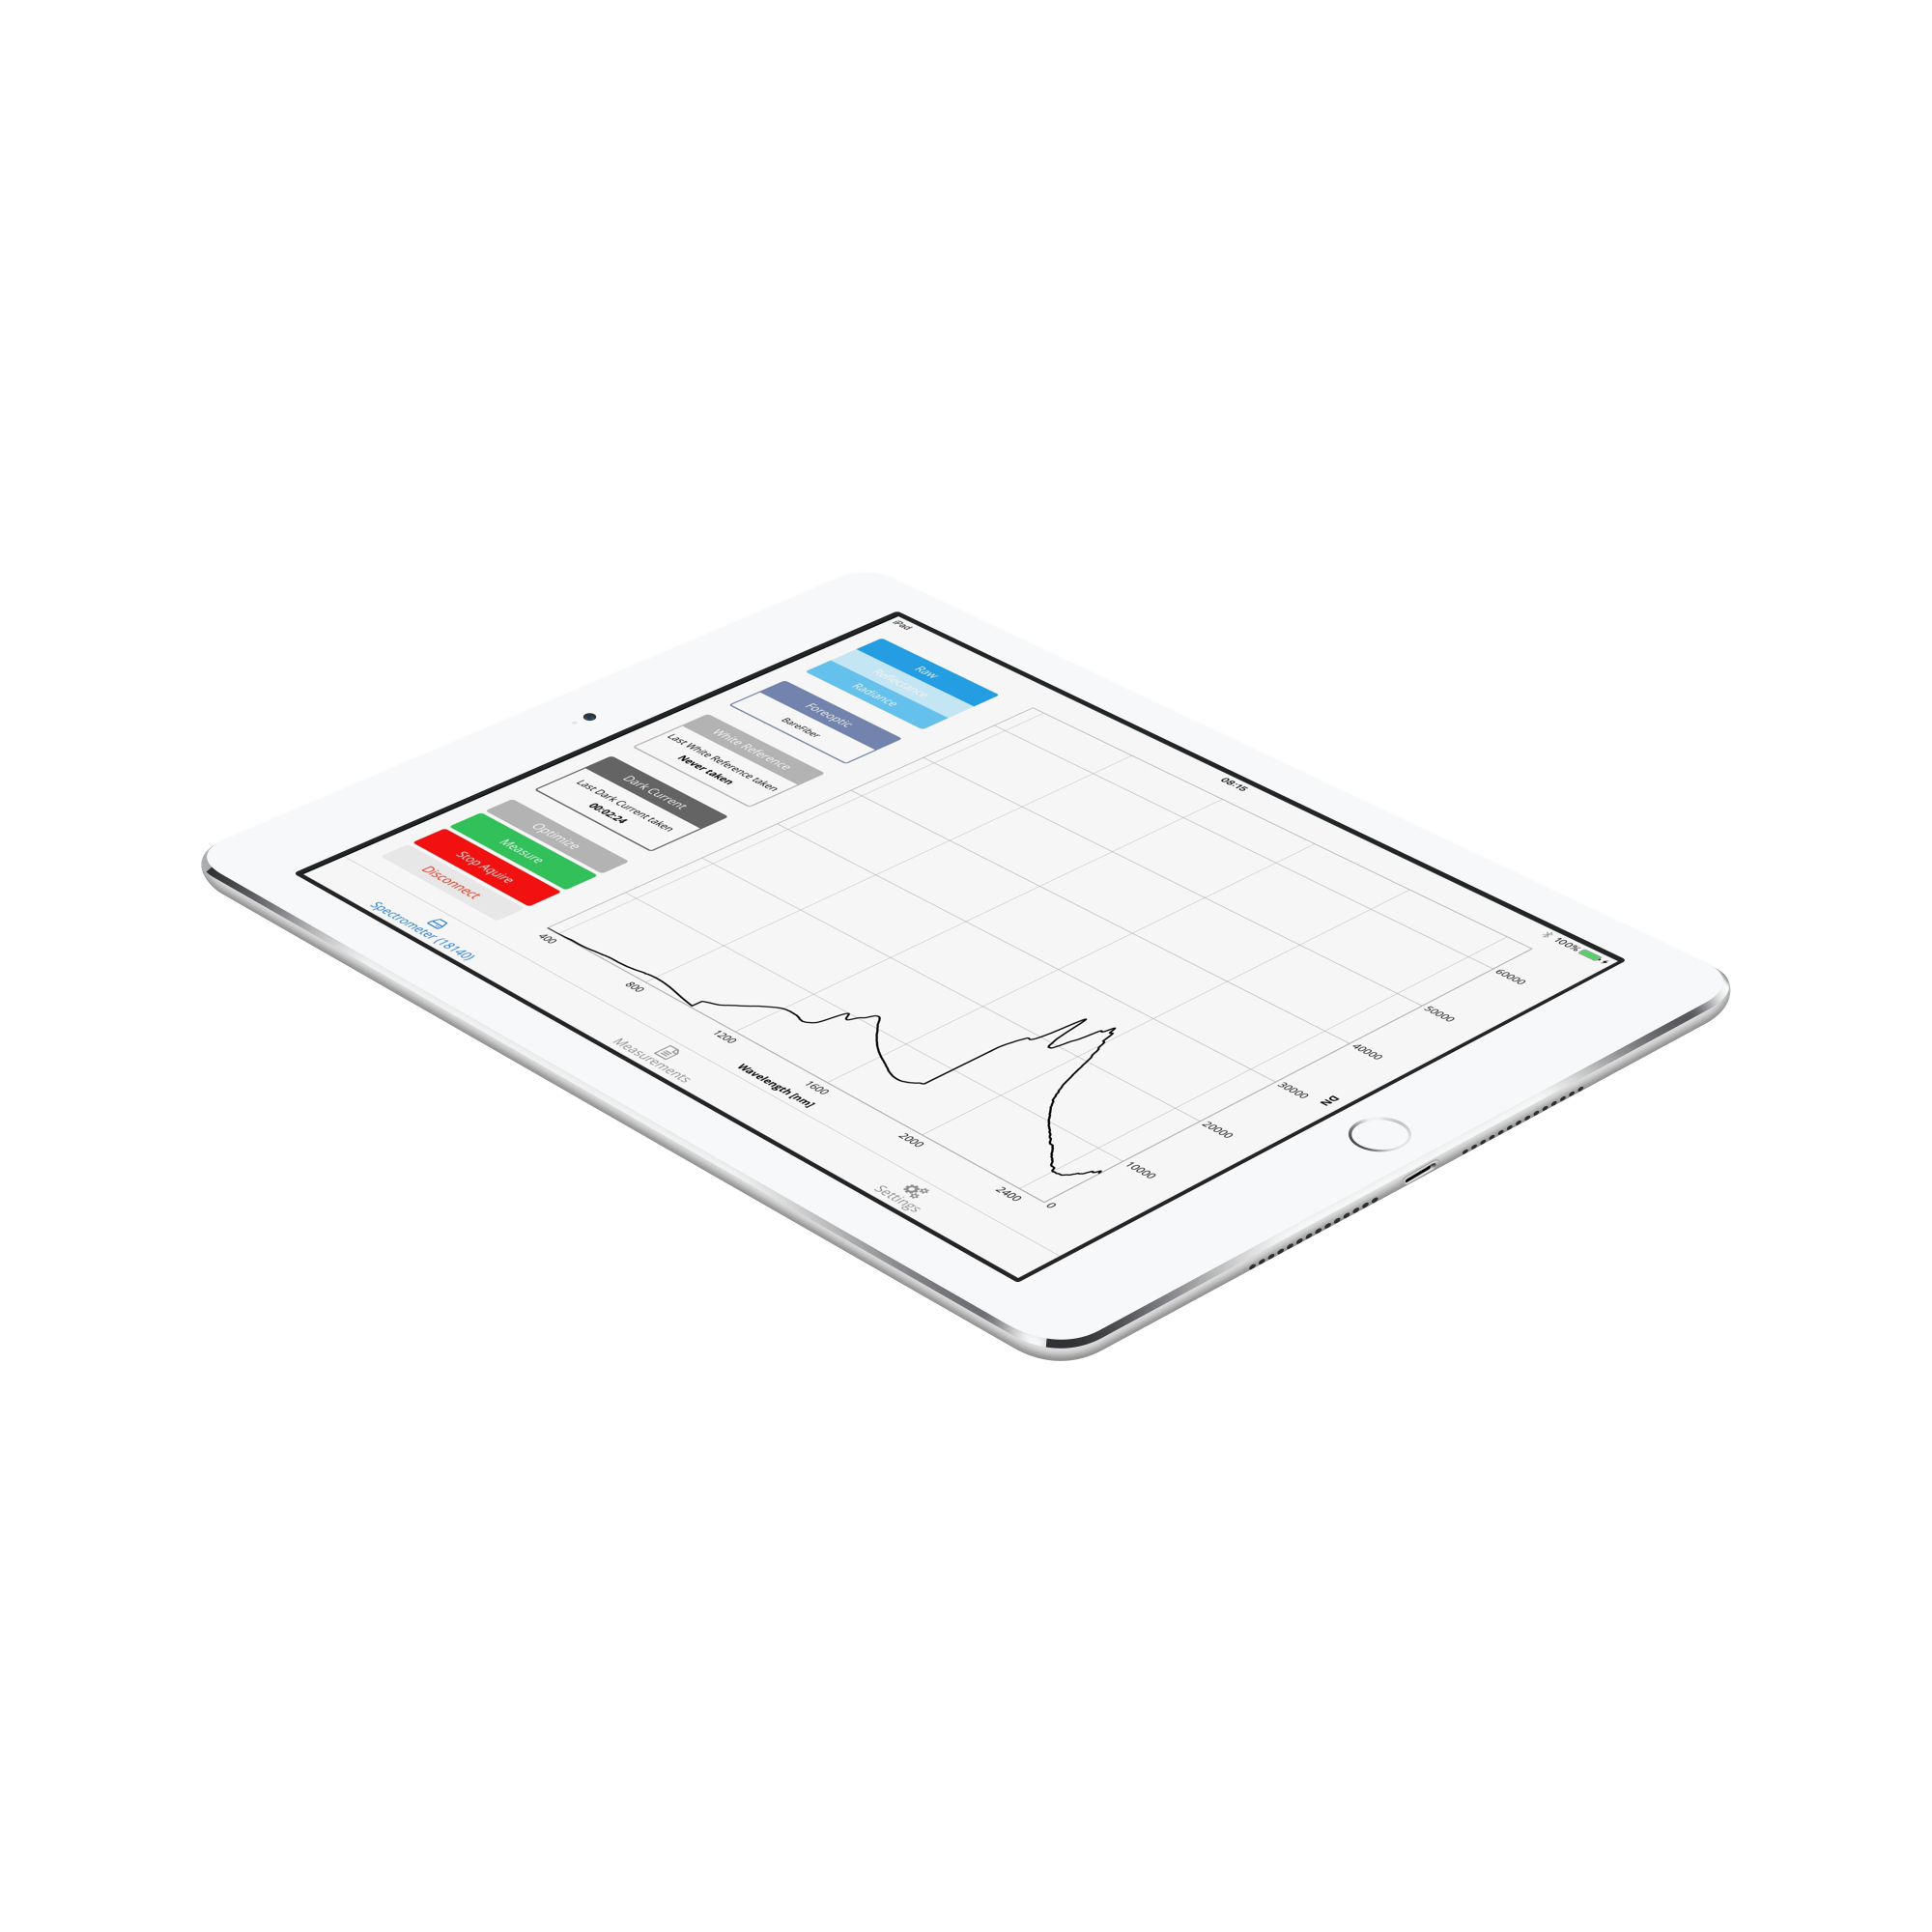
\includegraphics[scale=0.3]{images/ipadAir_Spektrometer}
		\end{center}
		
		\vfill
		\large{
			\hspace{-0.83cm} 
\includegraphics{images/fhnw_logo}\\
			\line(1,0){165}	

			\vspace{0.5cm}
			Dozent: \dozent \\
			\vspace{0.1cm}
			Auftraggeber:  \auftraggeber \\
			\vspace{0.5cm}
			\ort, \datum
		}
	\end{center}
\end{titlepage}

% Inhaltsverzeichnis
\pagenumbering{Roman}
\tableofcontents
\listoffigures 								% Abbildungsverzeichnis

% Abstract
\begin{abstract}

Das Hauptziel des Projektes ist, eine mobile Applikation zu erstellen, welche die RS\textsuperscript{3} Desktopl�sung von ASD abl�st. RS\textsuperscript{3} ist eine Software, welche die Verbindung zu einem Spektralmessger�t herstellt, Messungen ausl�sen sowie die Resultate anzeigen kann. Das bisherige System besteht aus einem Laptop inklusive RS\textsuperscript{3} Software, welche jeweils auf ein Spektrometer abgestimmt ist. Neu soll eine mobile App ausreichen, um mehrere Spektrometer ansprechen zu k�nnen. Die App soll Forschende unterst�tzen, Messungen direkt im Feld zu beurteilen und verwalten zu k�nnen. Die erstellten Messungen sollen abschliessend exportiert werden k�nnen, um diese am Computer weiterzuverwenden. 

\end{abstract}
\pagenumbering{arabic}

% Ausgangslage und Problemstellung
\chapter{Einleitung}

\section{Ziel der Arbeit} \label{ziel}
Das geologische Institut der Universit�t Z�rich betreibt zur Forschung vier Spektrometer der Firma ASD Inc. aus Colorado in den USA. Zu jedem Spektrometer liefert ASD einen Notebook mit installierter Software, um das  \gls{spectrometer} zu bedienen und Messungen auszuf�hren.

Ziel dieser Arbeit war, die Software \href{https://www.asdi.com/products-and-services/software/rs3}{RS\textsuperscript{3}} von ASD mit einer modernen Applikation f�r ein mobiles Device abzul�sen. Das Projektteam hat sich gemeinsam mit dem Kunden dazu entschieden, die Applikation f�r iOS Ger�te, im speziellen iPads, zu entwickeln.

\section{Hilfestellungen} \label{hilfestellungen}
Zur Umsetzung konnten verschiedene Hilfestellungen in Anspruch genommen werden. ASD bietet auf ihrer Webseite einen \href{http://support.asdi.com/Products/Products.aspx}{Download} mit einem Developer-Kit an. In dieser Dokumentation ist beschrieben, wie interessierte Entwickler mittels eines TCP-Servers, der auf dem Spektrometer betrieben wird, selbst Applikationen entwickeln k�nnen. Die Dokumentation enth�lt ausf�hrliche Informationen zu Verbindungsparameter, R�ckgabetypen und Dateiformaten.

Weiter konnte auf das \href{https://github.com/ahueni/SPECCHIO}{GitHub Repository} der SPECCHIO-Datenbank zur�ckgegriffen werden. In dieser Applikation wurden verschiedenste Berechnungen und Manipulationen mit Spektraldaten oder Spektraldateien bereits in Java programmiert.

\section{Erreichtes} \label{erreichtes}
Die Applikation wurde mit den definierten Grundanforderungen vollst�ndig umgesetzt. Der Benutzer kann, sofern das iPad mit dem Spektrometer �ber WLAN verbunden ist, das Spektrometer bedienen und Messungen ausf�hren. Es wurde speziell darauf geachtet, den Messablauf einfacher und f�r den Benutzer intuitiver zu gestalten. Die Grundansicht wurde nahezu von der bestehenden Software �bernommen. Somit sollte es f�r die Benutzer keine zu grosse Umstellung sein.

Weiter wurde darauf geachtet, die Applikation in Zukunft noch weiter zu entwickeln. Die Architektur wurde stark strukturiert, damit auch Personen, die noch nicht mit dem Projekt vertraut sind, eine Weiterentwicklung vornehmen k�nnen. 

\section{Leserf�hrung} \label{leserfuehrung}
Dieses Dokument beschreibt die Erarbeitung eines Informatik Projektes 6 der Fachhochschule Nordwestschweiz. Die Dokumentation ist in einen theoretischen und einen praktischen Teil aufgeteilt. Im theoretischen Teil wird nur kurz erkl�rt was ein Spektrometer genau misst und wie die Daten berechnet und abgespeichert werden. Im praktischen Teil wird vor allem die Softwarearchitektur und die konkrete Umsetzung genau beschrieben.


\end{document}